\begin{comment}
\addbibresource{referencias/Referencias.bib}
\end{comment}

\section{Resultados}
\label{sc:resultados}

% A continuación se ilustran los resultados obtenidos por el análisis de las funciones de atenuación. Para cada caso se presentarán perfiles para las deformaciones en x ($\varepsilon_x$)
\subsection{Caso de estudio 1: Placa a tensión}
% Para el caso de la placa a tensión se evaluarán perfiles de deformaciones en cada dirección, para ello, se disponen de dos perfiles por dirección, uno en el que los puntos de evaluación se encuentran dentro de una distancia $Lr=6l$ desde los bordes del dominio y otro en el que los puntos de evaluación se encuentran en su mayoría en la zona interior del dominio. Para este caso se evaluará perfiles en $x=0.019$, $x=0.019$, $x=2.519$, $y=0.019$ y $y=2.519$
	\subsubsection{\texorpdfstring{$x=0.019$}{x=0.019}}

		\begin{figure}
		    \centering
		    \sffamily
		    \begin{subfigure}{0.48\textwidth}
		    \centering
		        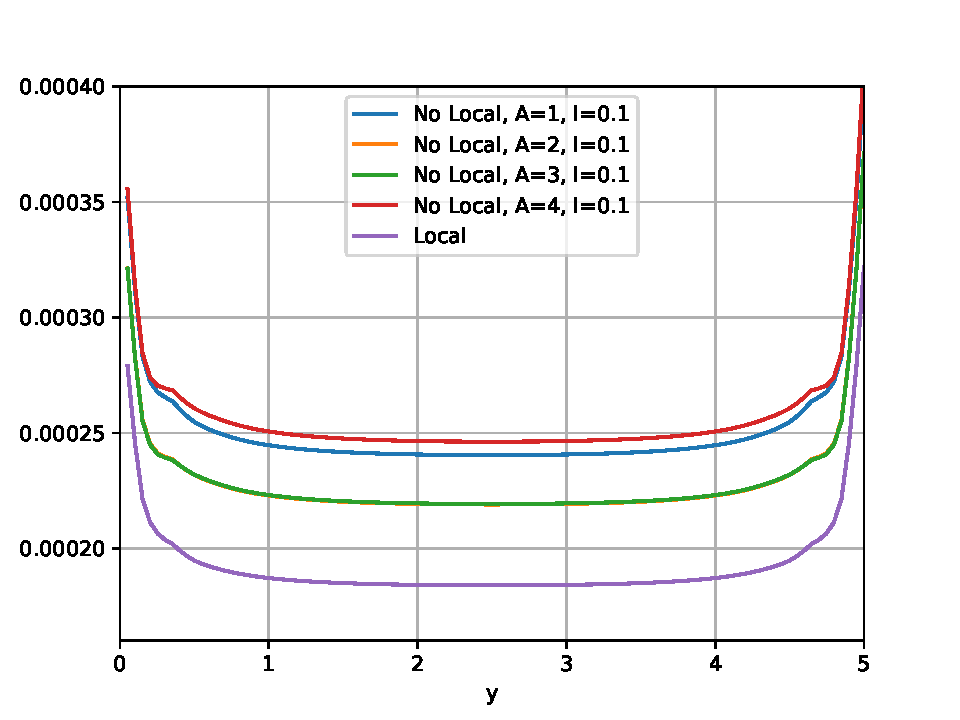
\includegraphics[width=\textwidth]{figuras/Placa/Perfiles/X/X0.1_0.019.pdf}
		        \caption{$l=0.1$}
		        \label{fig:perfilesX0019.01}
		    \end{subfigure}
		    \begin{subfigure}{0.48\textwidth}
		    \centering
		        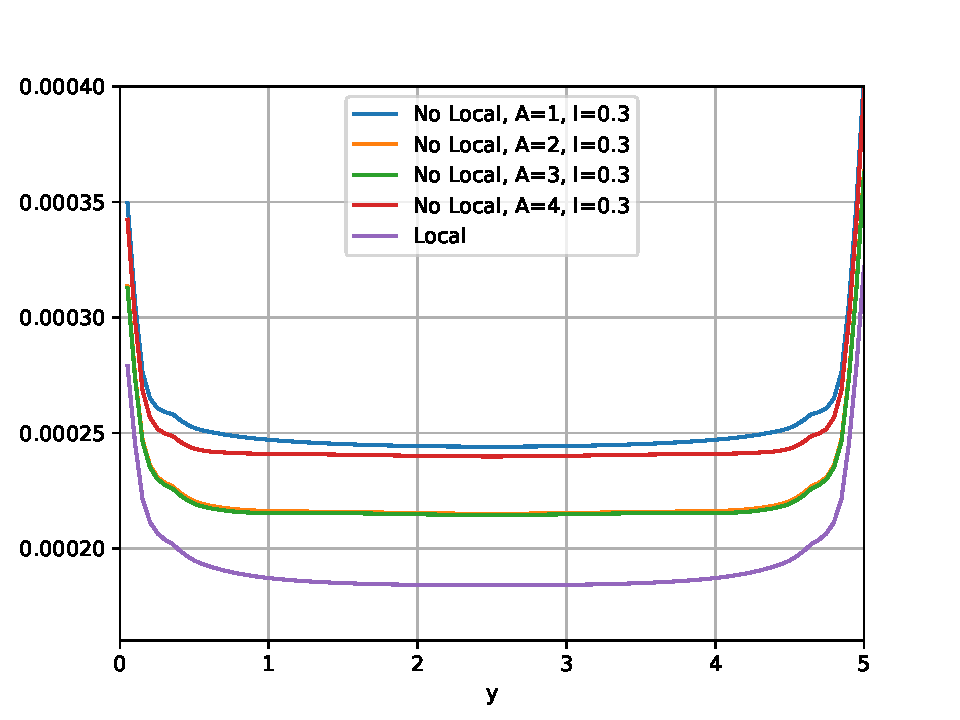
\includegraphics[width=\textwidth]{figuras/Placa/Perfiles/X/X0.3_0.019.pdf}
		        \caption{$l=0.3$}
		        \label{fig:perfilesX0019.03}
		    \end{subfigure}
		    \quad
		    \begin{subfigure}{0.48\textwidth}
		    \centering
		        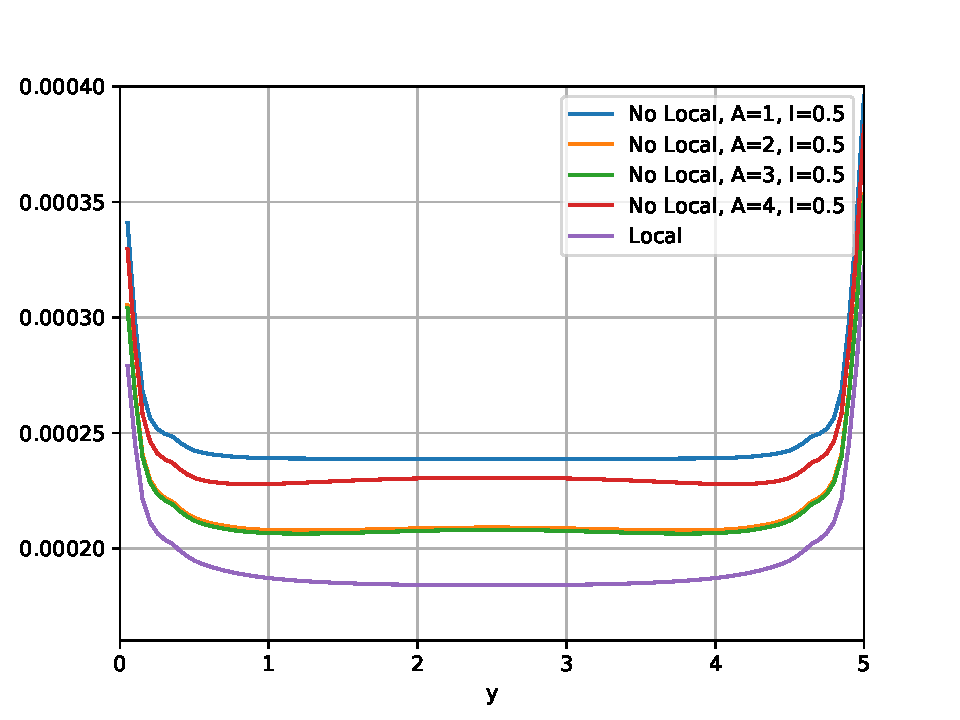
\includegraphics[width=\textwidth]{figuras/Placa/Perfiles/X/X0.5_0.019.pdf}
		        \caption{$l=0.5$}
		        \label{fig:perfilesX0019.05}
		    \end{subfigure}
		    \begin{subfigure}{0.48\textwidth}
		    \centering
		        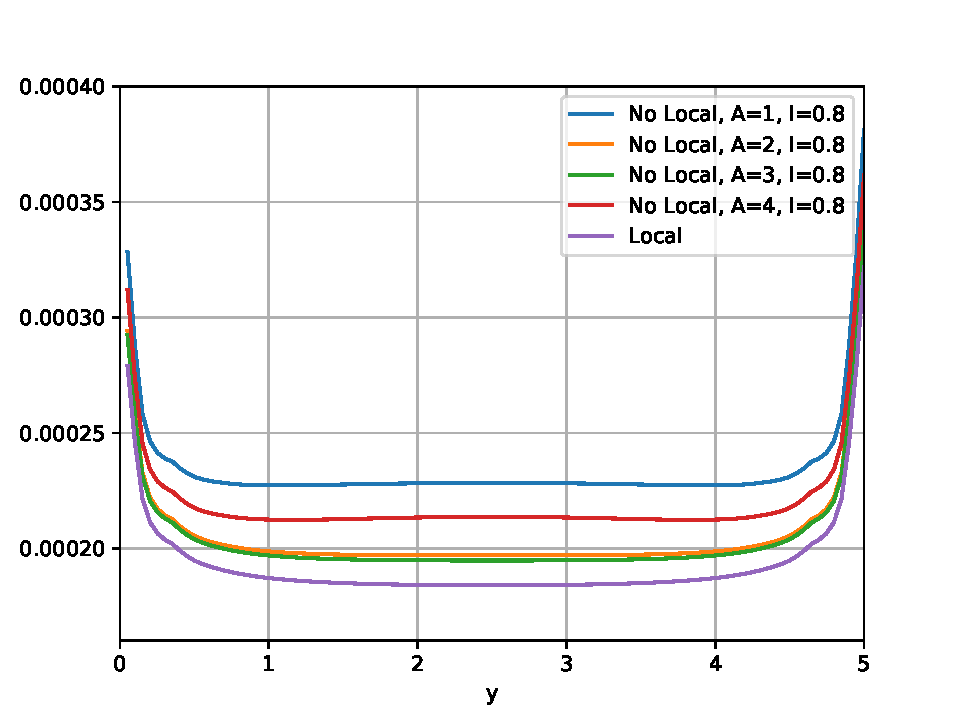
\includegraphics[width=\textwidth]{figuras/Placa/Perfiles/X/X0.8_0.019.pdf}
		        \caption{$l=0.8$}
		        \label{fig:perfilesX0019.08}
		    \end{subfigure}
		    \caption{Perfiles de $\varepsilon_x$ en $x=0.019$}
		    \label{fig:perfilesX0019}
		\end{figure}
	\begin{wrapfigure}{l}{0.3\textwidth}
		\sffamily
		\begin{center}
			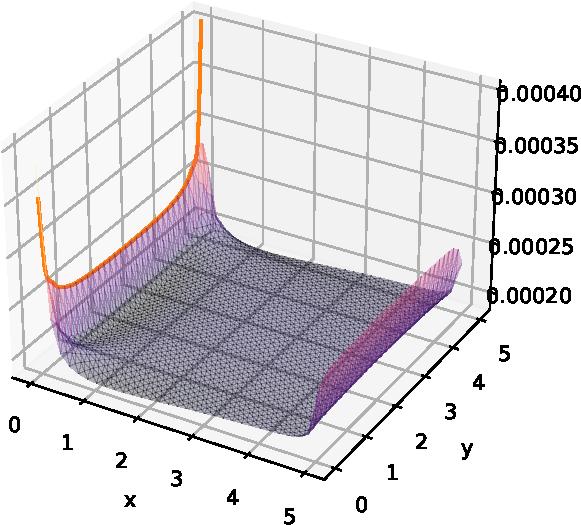
\includegraphics[width=0.3\textwidth]{figuras/Placa/defx_bonita_X0.019.pdf}
		\end{center}
		\caption{Ubicación del perfil}
		\label{fig:defxbonitax0019}
	\end{wrapfigure}
	Como se nota en la figura \ref{fig:defxbonitax0019}, este perfil se está graficando prácticamente en el borde del dominio, lo cual, significa que los valores calculados se encuentran a una distancia menor que $Lr=6l$ del borde del dominio. En este caso se observa que el perfil para las deformaciones locales se encuentra siempre por debajo de las deformaciones no locales.

	Para esta gráfica y las siguientes se tiene una convención de funciones, la función A=1 corresponde a la función de atenuación 1 expuesta en el capítulo \ref{sc:teoria}. Como referente, la función 1 es la función biexponencial, la función 2 es la función lineal, la función 3 es la función cuadrática y la función 4 es la función modificada. Se puede evidenciar que cuando $l$ es pequeño no existe una diferencia relevante entre las deformaciones obtenidas por las funciones 2 y 3. Para este caso se puede apreciar que mediante la función modificada se pueden obtener deformaciones mayores solo si $l$ es pequeño.


	\subsubsection{\texorpdfstring{$x=2.519$}{x=2.519}}
		\begin{figure}
		    \centering
		    \sffamily
		    \begin{subfigure}{0.48\textwidth}
		    \centering
		        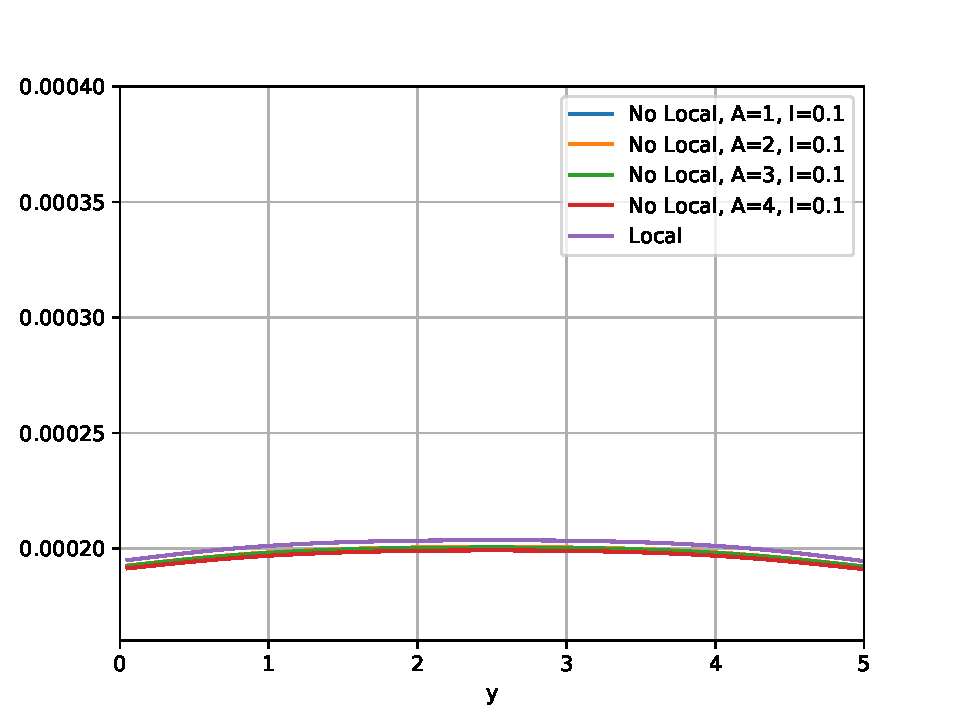
\includegraphics[width=\textwidth]{figuras/Placa/Perfiles/X/X0.1_2.519.pdf}
		        \caption{$l=0.1$}
		        \label{fig:perfilesX0259.01}
		    \end{subfigure}
		    \begin{subfigure}{0.48\textwidth}
		    \centering
		        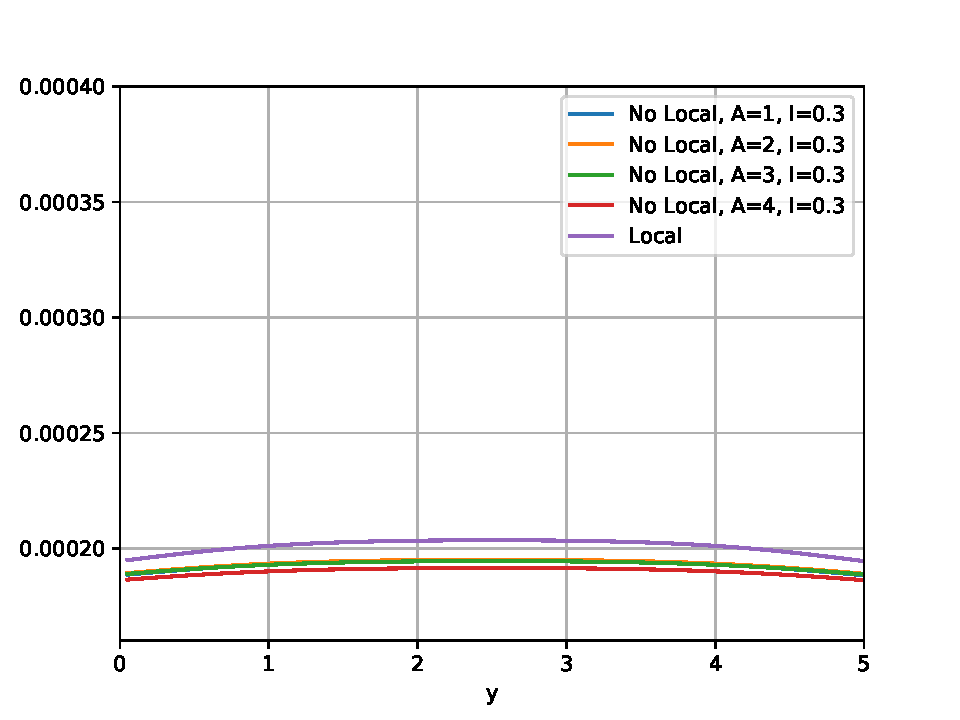
\includegraphics[width=\textwidth]{figuras/Placa/Perfiles/X/X0.3_2.519.pdf}
		        \caption{$l=0.3$}
		        \label{fig:perfilesX0259.03}
		    \end{subfigure}
		    \quad
		    \begin{subfigure}{0.48\textwidth}
		    \centering
		        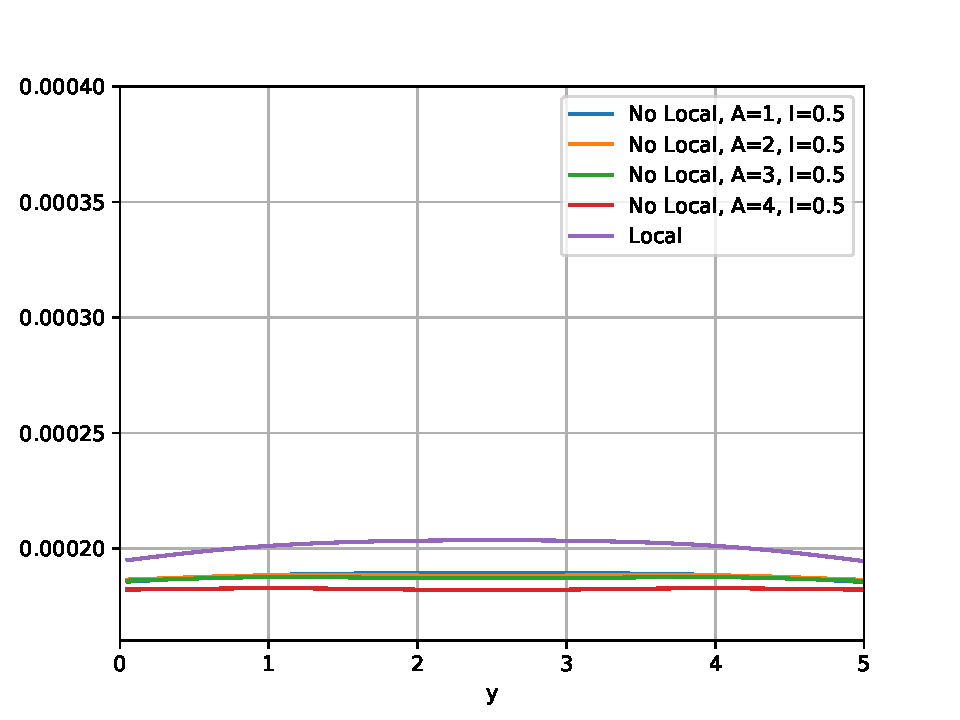
\includegraphics[width=\textwidth]{figuras/Placa/Perfiles/X/X0.5_2.519.pdf}
		        \caption{$l=0.5$}
		        \label{fig:perfilesX0259.05}
		    \end{subfigure}
		    \begin{subfigure}{0.48\textwidth}
		    \centering
		        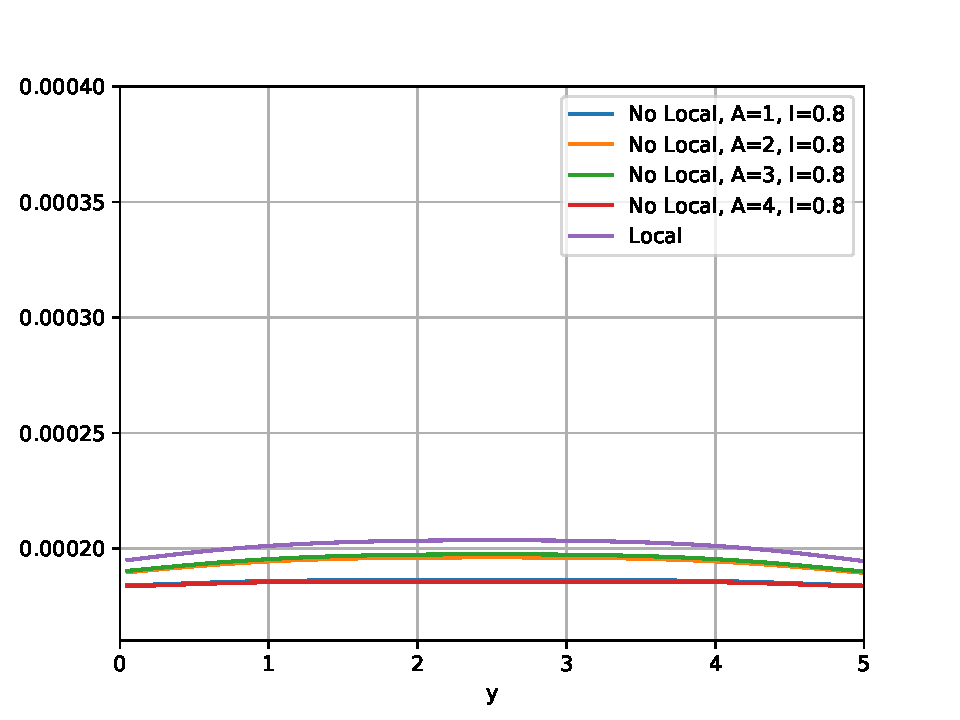
\includegraphics[width=\textwidth]{figuras/Placa/Perfiles/X/X0.8_2.519.pdf}
		        \caption{$l=0.8$}
		        \label{fig:perfilesX0259.08}
		    \end{subfigure}
		    \caption{Perfiles de $\varepsilon_x$ en $x=2.519$}
		    \label{fig:perfilesX0259}
		\end{figure}
	\begin{wrapfigure}{l}{0.3\textwidth}
		\sffamily
		\begin{center}
			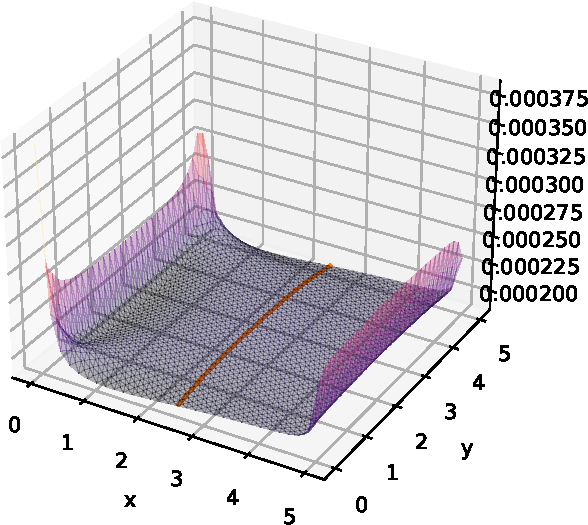
\includegraphics[width=0.3\textwidth]{figuras/Placa/defx_bonita_X2.519.pdf}
		\end{center}
		\caption{Ubicación del perfil}
		\label{fig:defxbonitax2519}
	\end{wrapfigure}
	Para este caso se realizó el perfil en la mitad del dominio, por lo que la mayoría de los puntos están en la parte interior del dominio. En las zonas interiores del dominio se espera que los resultados obtenidos por la teoría local y no local sigan el mismo patrón \parencite{Pisano2009}.

	Como se muestran los resultados para las deformaciones en x, en este perfil no se debería evidenciar una variación severa en los resultados. Como se aprecia en la figura \ref{fig:perfilesX0259.01} se puede ver que los resultados obtenidos se agrupan por debajo de la solución local, mientras que en la figura \ref{fig:perfilesX0259.08} se puede apreciar que las soluciones se agrupan en diferentes zonas.\newline\newline\newline\newline\newline\newline



	\subsubsection{\texorpdfstring{$y=0.019$}{y=0.019}}
		\begin{figure}
		    \centering
		    \sffamily
		    \begin{subfigure}{0.48\textwidth}
		    \centering
		        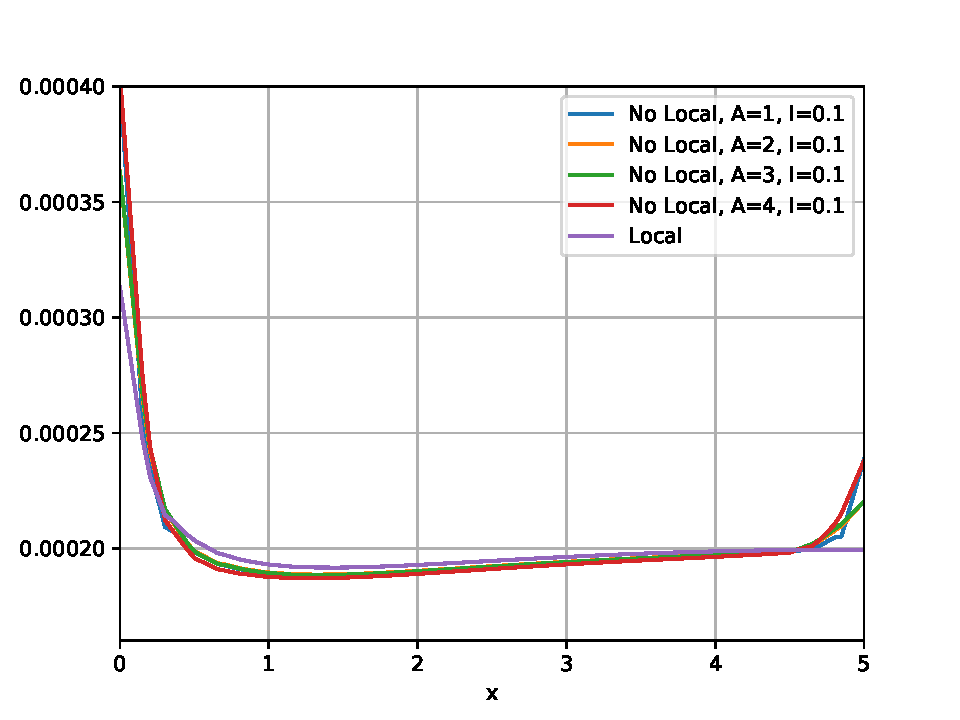
\includegraphics[width=\textwidth]{figuras/Placa/Perfiles/Y/Y0.1_0.019.pdf}
		        \caption{$l=0.1$}
		        \label{fig:perfilesY0019.01}
		    \end{subfigure}
		    \begin{subfigure}{0.48\textwidth}
		    \centering
		        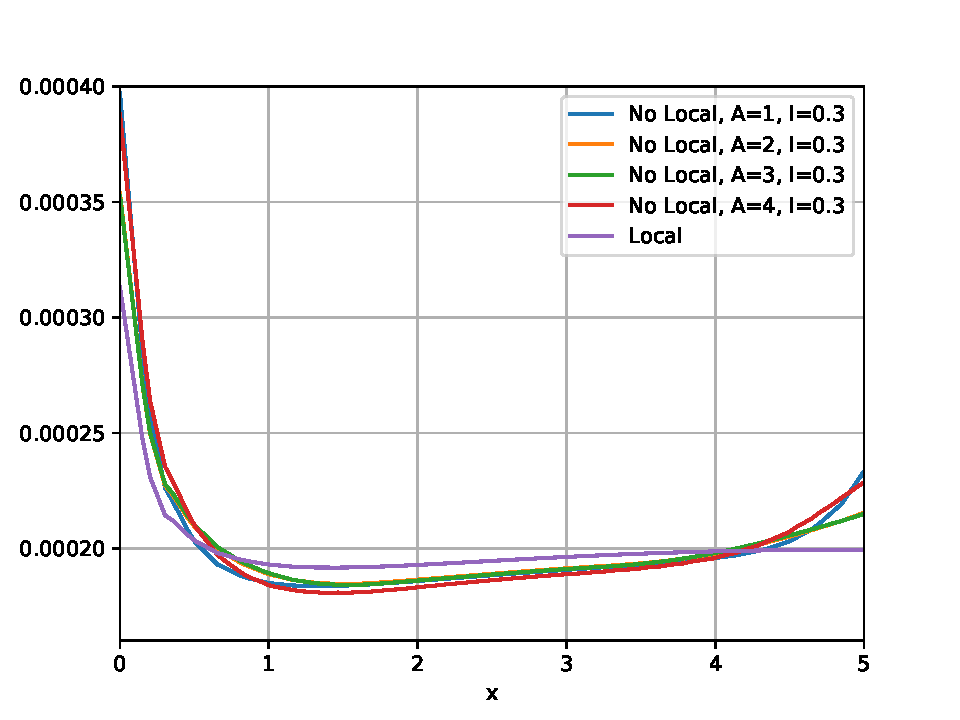
\includegraphics[width=\textwidth]{figuras/Placa/Perfiles/Y/Y0.3_0.019.pdf}
		        \caption{$l=0.3$}
		        \label{fig:perfilesY0019.03}
		    \end{subfigure}
		    \quad
		    \begin{subfigure}{0.48\textwidth}
		    \centering
		        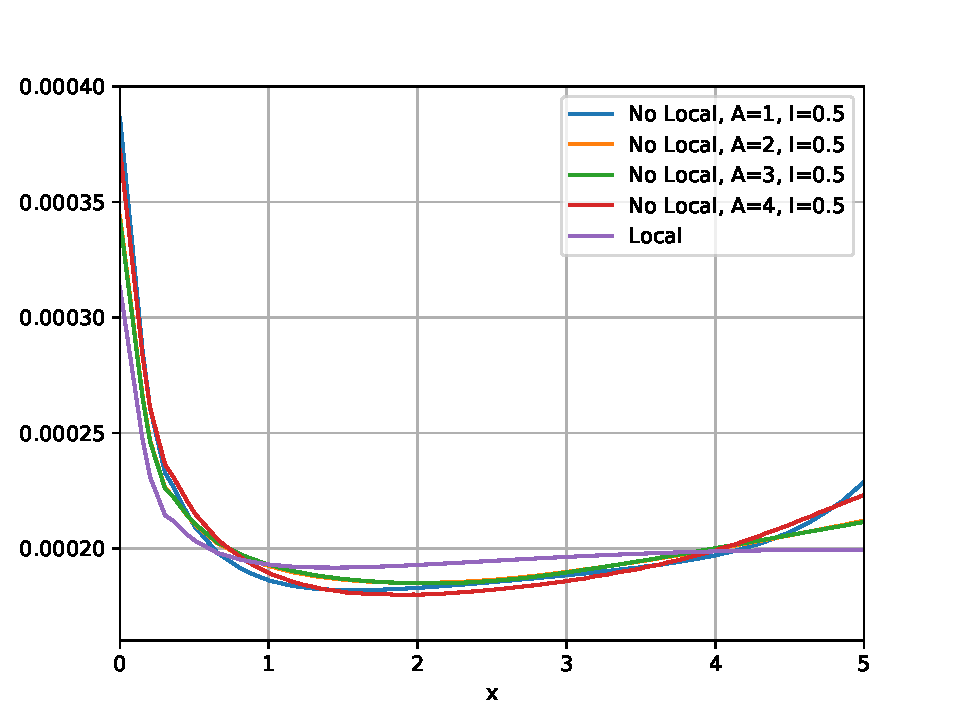
\includegraphics[width=\textwidth]{figuras/Placa/Perfiles/Y/Y0.5_0.019.pdf}
		        \caption{$l=0.5$}
		        \label{fig:perfilesY0019.05}
		    \end{subfigure}
		    \begin{subfigure}{0.48\textwidth}
		    \centering
		        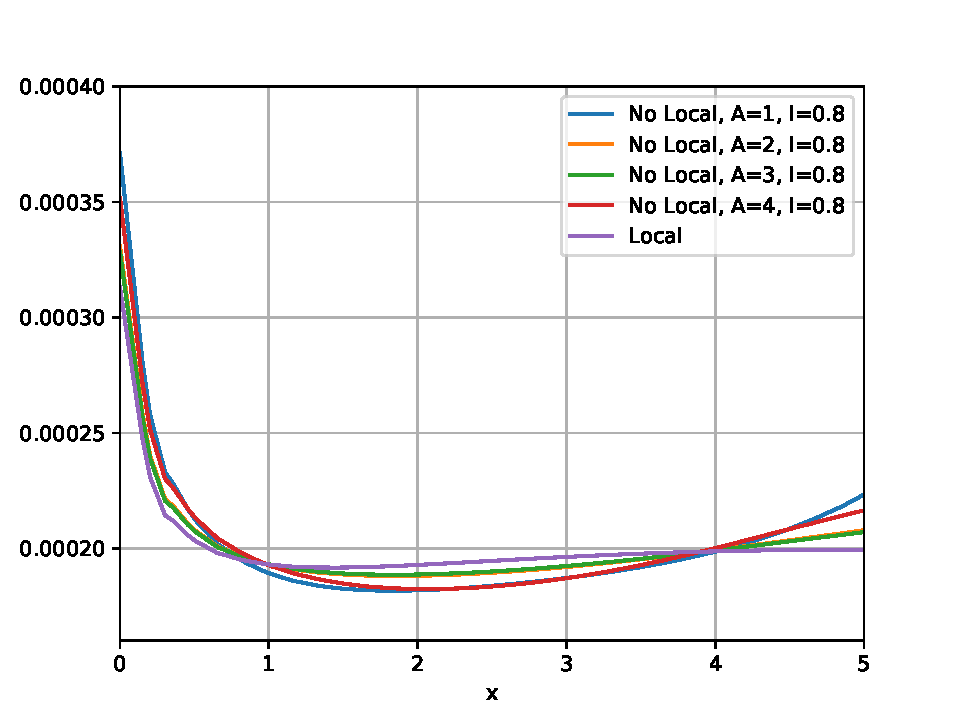
\includegraphics[width=\textwidth]{figuras/Placa/Perfiles/Y/Y0.8_0.019.pdf}
		        \caption{$l=0.8$}
		        \label{fig:perfilesY0019.08}
		    \end{subfigure}
		    \caption{Perfiles de $\varepsilon_x$ en $y=0.019$}
		    \label{fig:perfilesY0019}
		\end{figure}
	\begin{wrapfigure}{l}{0.3\textwidth}
		\sffamily
		\begin{center}
			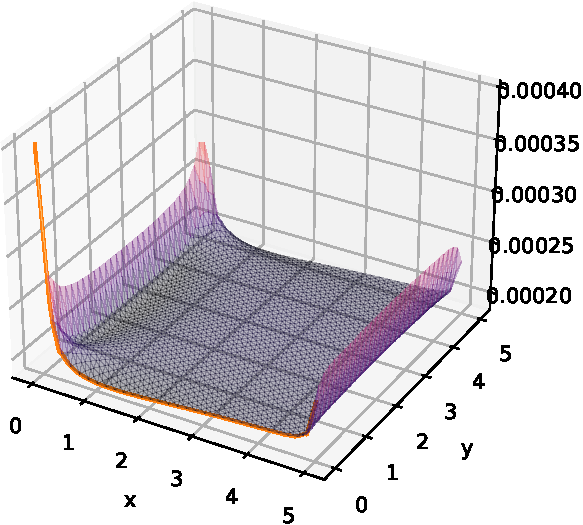
\includegraphics[width=0.3\textwidth]{figuras/Placa/defx_bonita_Y0.019.pdf}
		\end{center}
		\caption{Ubicación del perfil}
		\label{fig:defxbonitay0019}
	\end{wrapfigure}
	En este caso se evalúan los resultados nuevamente a una distancia desde el borde menor que $Lr$, en este caso se evalúan los cambios de la deformación variando x, lo cual provee una mejor visualización del fenómeno. Como peculiaridad se aprecia que al obtener las deformaciones no locales se obtienen deformaciones más altas en los bordes donde se aplican las condiciones de borde, mientras que en la zona central del dominio las deformaciones obtenidas por la teoría no local tienden a ser menores que las obtenidas por la teoría local.

	Como se mencionó en el capítulo \ref{sc:metodos} los valores para $l$ fueron escogidos para obtener resultados donde la distancia $Lr$ fuera lo suficientemente grande para abarcar con todo el dominio. En el caso de la figura \ref{fig:perfilesY0019.01} y \ref{fig:perfilesY0019.03} $Lr=0.6,1.8$ respectivamente, por lo tanto, $Lr<a/2$. En estos dos perfiles se puede apreciar que las deformaciones que estén entre $Lr<=x<=a-Lr$ presentan un comportamiento paralelo a la solución local. Para las zonas donde no se cumple esta condición se presenta el comportamiento de picos que se hace más pronunciado mientras $l$ es más grande. Para el caso de las figuras \ref{fig:perfilesY0019.05} y \ref{fig:perfilesY0019.08} ase tiene un $Lr>a/2$, por lo que no se puede evidenciar el comportamiento paralelo que se mostró anteriormente.



	\subsubsection{\texorpdfstring{$y=2.519$}{y=2.519}}
		\begin{figure}
		    \centering
		    \sffamily
		    \begin{subfigure}{0.48\textwidth}
		    \centering
		        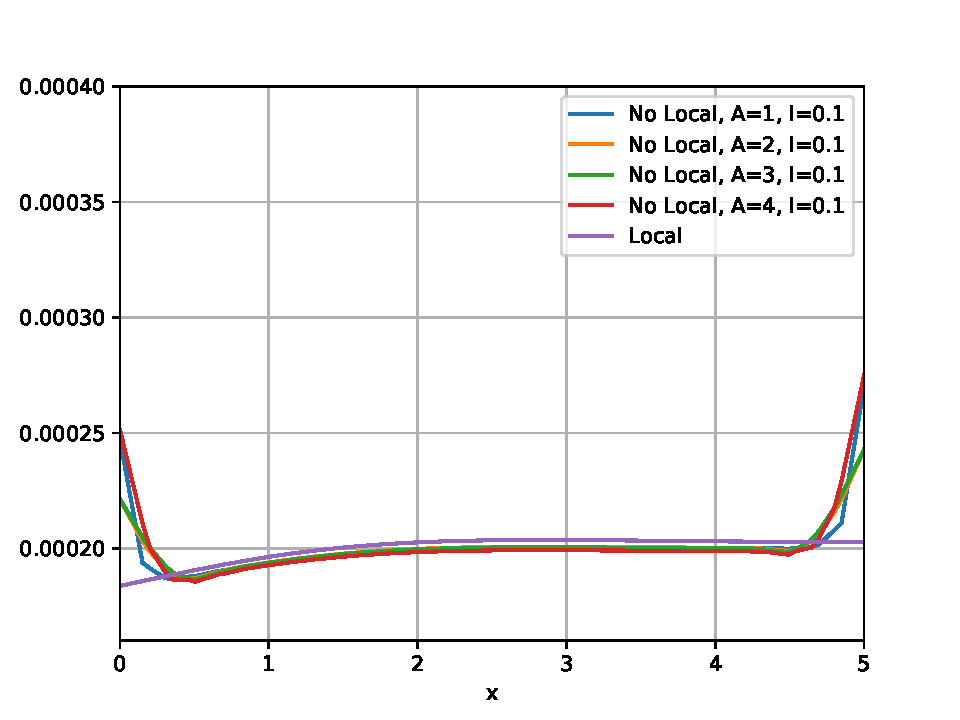
\includegraphics[width=\textwidth]{figuras/Placa/Perfiles/Y/Y0.1_2.519.pdf}
		        \caption{$l=0.1$}
		        \label{fig:perfilesY0259.01}
		    \end{subfigure}
		    \begin{subfigure}{0.48\textwidth}
		    \centering
		        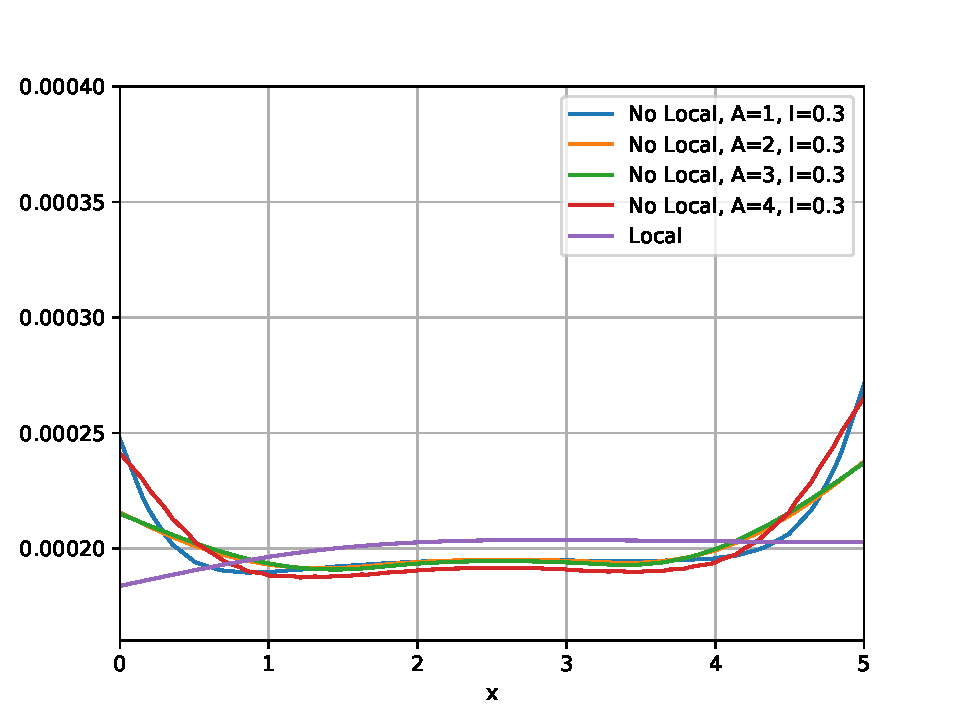
\includegraphics[width=\textwidth]{figuras/Placa/Perfiles/Y/Y0.3_2.519.pdf}
		        \caption{$l=0.3$}
		        \label{fig:perfilesY0259.03}
		    \end{subfigure}
		    \quad
		    \begin{subfigure}{0.48\textwidth}
		    \centering
		        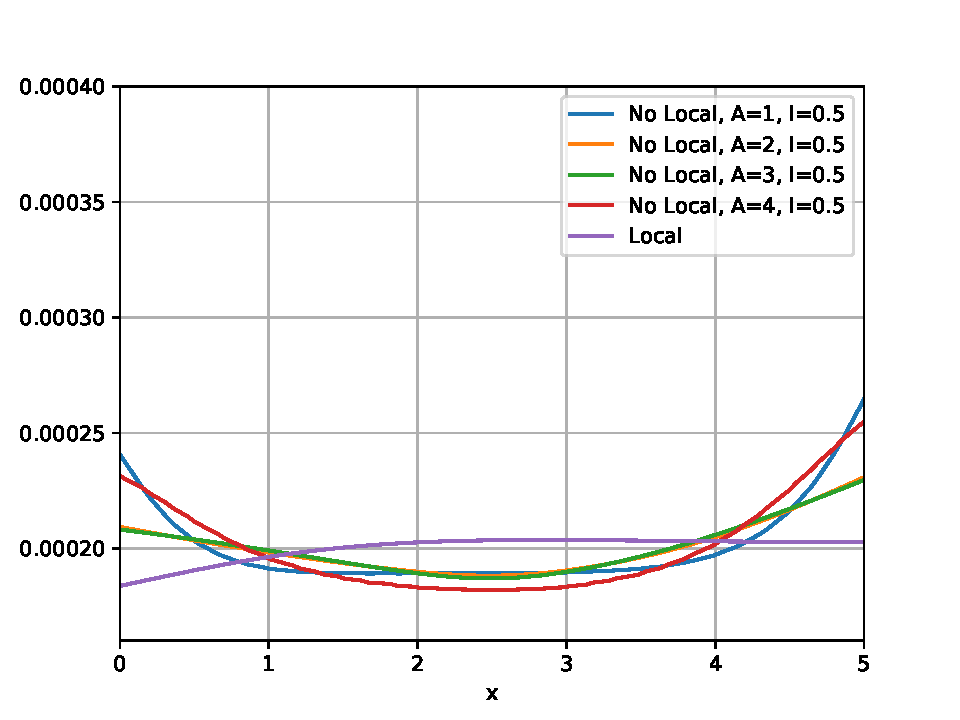
\includegraphics[width=\textwidth]{figuras/Placa/Perfiles/Y/Y0.5_2.519.pdf}
		        \caption{$l=0.5$}
		        \label{fig:perfilesY0259.05}
		    \end{subfigure}
		    \begin{subfigure}{0.48\textwidth}
		    \centering
		        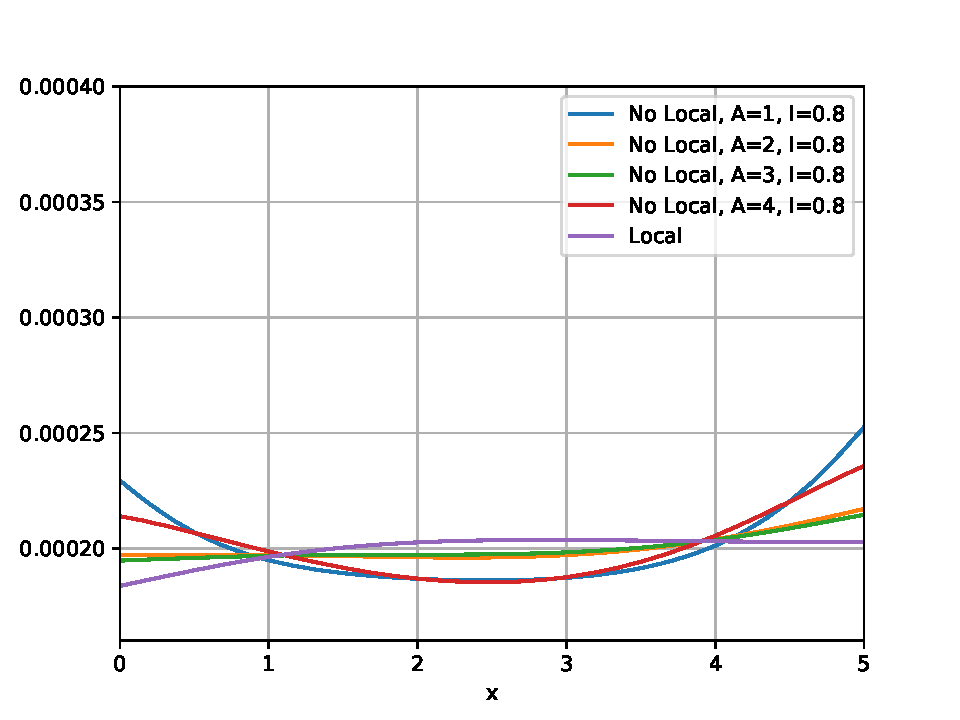
\includegraphics[width=\textwidth]{figuras/Placa/Perfiles/Y/Y0.8_2.519.pdf}
		        \caption{$l=0.8$}
		        \label{fig:perfilesY0259.08}
		    \end{subfigure}
		    \caption{Perfiles de $\varepsilon_x$ en $y=2.519$}
		    \label{fig:perfilesY0259}
		\end{figure}
	\begin{wrapfigure}{l}{0.3\textwidth}
		\sffamily
		\begin{center}
			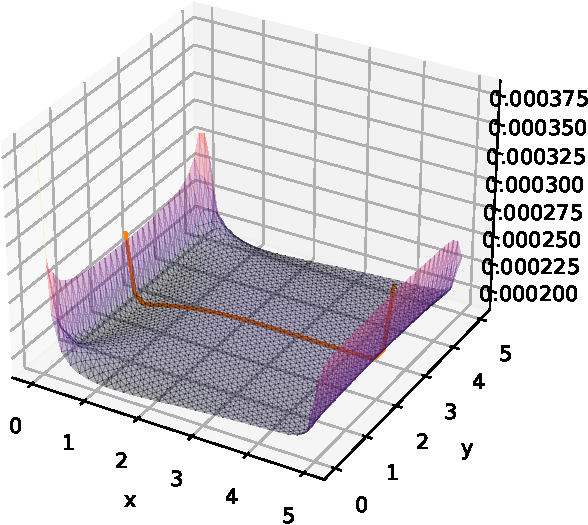
\includegraphics[width=0.3\textwidth]{figuras/Placa/defx_bonita_Y2.519.pdf}
		\end{center}
		\caption{Ubicación del perfil}
		\label{fig:defxbonitay2519}
	\end{wrapfigure}
	En este caso se evalúan los resultados a una distancia desde el borde mayor que $Lr$, en este caso se evalúan los cambios de la deformación variando x, lo cual provee una mejor visualización del fenómeno. En estos perfiles se puede evidenciar el comportamiento de la solución al momento de aumentar el factor $l$. En el caso de la figura \ref{fig:perfilesY0259.01} y \ref{fig:perfilesY0259.03} $Lr=0.6,1.8$ lo que lleva a pensar que las deformaciones en la zona interior sean paralelas a las obtenidas por la teoría local. En este caso que l es pequeño se evidencia que los resultados para cada una de las funciones son similares.

	En el caso de los perfiles donde $Lr>a/2$ no es posible evidenciar el comportamiento paralelo. Mas aún esto lleva a pensar en la existencia de puntos de inflexión donde la teoría no local producirá deformaciones mayores (y por lo tanto esfuerzos mayores) que se ubican a una distancia $Lr$ del borde del dominio. En el caso en el que $Lr$ no pueda desarrollarse completamente en el dominio, estos puntos de inflexión se juntan e invierten, lo que genera una superficie de esfuerzos diferente para cada función de atenuación.


\subsection{Caso de estudio 2: Barra a tensión}
	\subsubsection{\texorpdfstring{$y=0.5$}{y=0.5}}
		\begin{figure}
		    \centering
		    \sffamily
		    \begin{subfigure}{0.48\textwidth}
		    \centering
		        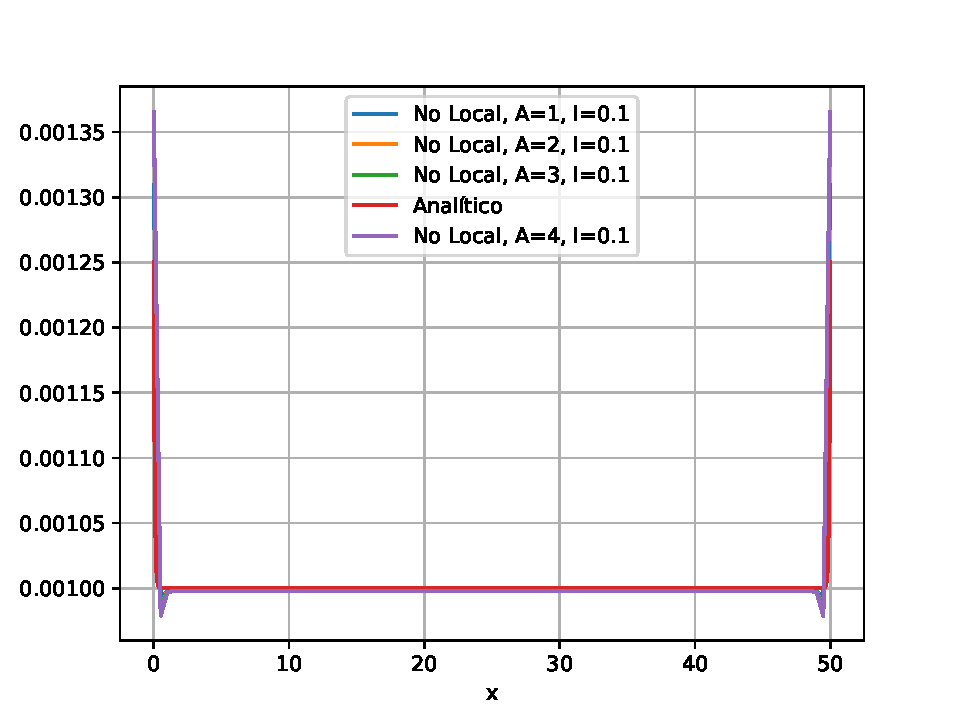
\includegraphics[width=\textwidth]{figuras/Barra/Perfiles/Y/Y0.1_0.5.pdf}
		        \caption{$l=0.1$}
		        \label{fig:perfilesbarraY05.01}
		    \end{subfigure}
		    \begin{subfigure}{0.48\textwidth}
		    \centering
		        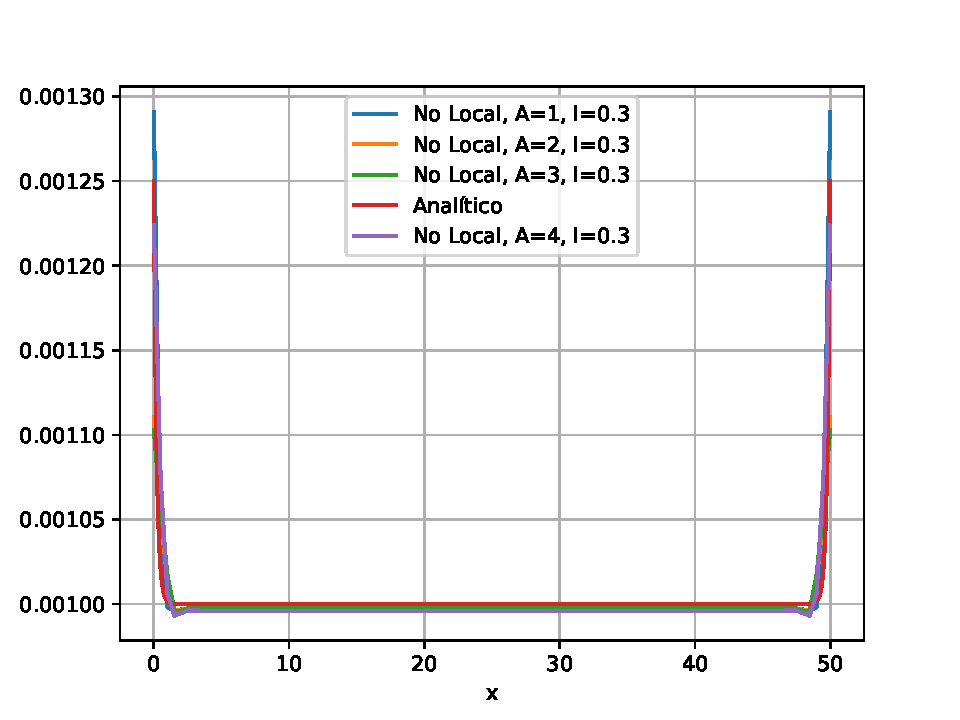
\includegraphics[width=\textwidth]{figuras/Barra/Perfiles/Y/Y0.3_0.5.pdf}
		        \caption{$l=0.3$}
		        \label{fig:perfilesbarraY05.03}
		    \end{subfigure}
		    \quad
		    \begin{subfigure}{0.48\textwidth}
		    \centering
		        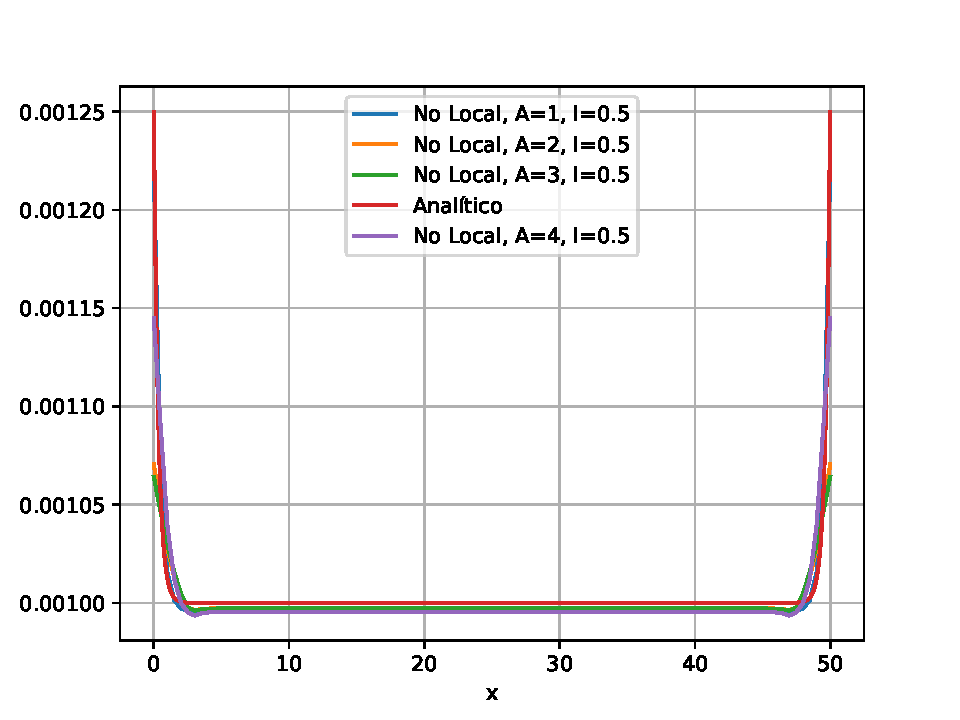
\includegraphics[width=\textwidth]{figuras/Barra/Perfiles/Y/Y0.5_0.5.pdf}
		        \caption{$l=0.5$}
		        \label{fig:perfilesbarraY05.05}
		    \end{subfigure}
		    \begin{subfigure}{0.48\textwidth}
		    \centering
		        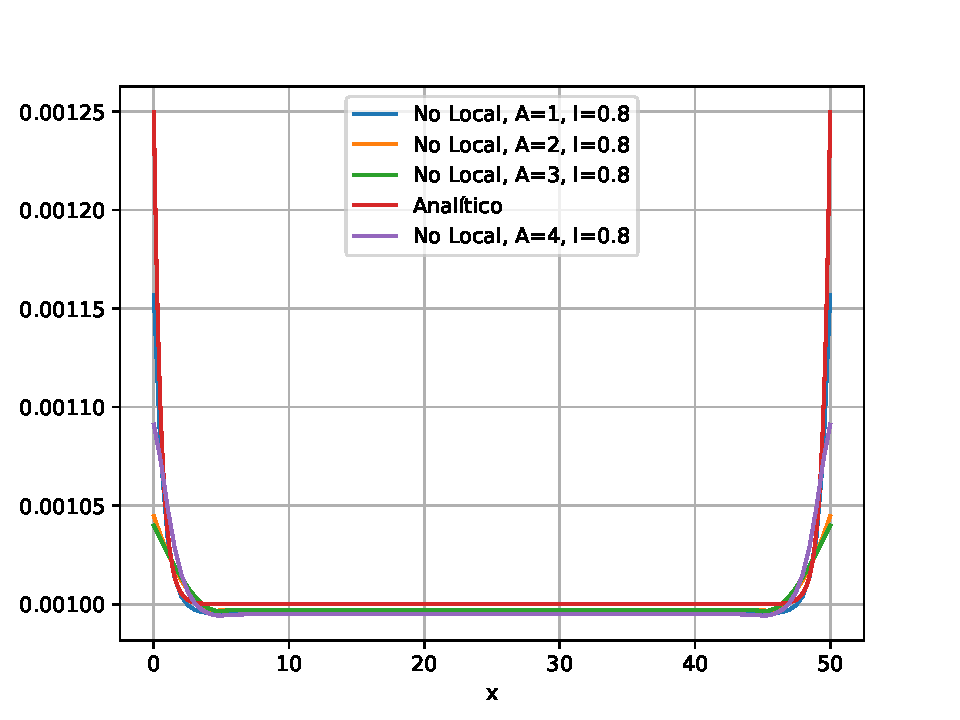
\includegraphics[width=\textwidth]{figuras/Barra/Perfiles/Y/Y0.8_0.5.pdf}
		        \caption{$l=0.8$}
		        \label{fig:perfilesbarraY05.08}
		    \end{subfigure}
		    \caption{Perfiles de $\varepsilon$ en $y=0.5$}
		    \label{fig:perfilesbarraY05}
		\end{figure}
	\begin{wrapfigure}{l}{0.3\textwidth}
		\sffamily
		\begin{center}
			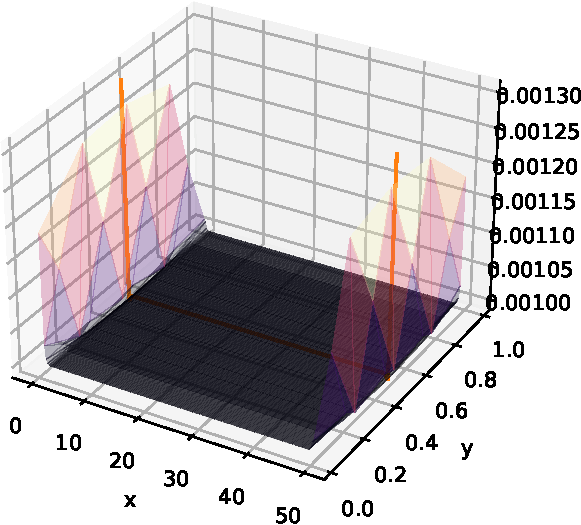
\includegraphics[width=0.3\textwidth]{figuras/Barra/defx_bonita_Y0.5.pdf}
		\end{center}
		\caption{Ubicación del perfil}
		\label{fig:defxbonitay05}
	\end{wrapfigure}
	En la figura \ref{fig:perfilesbarraY05} se muestra la comparación entre los resultados obtenidos contra la solución analítica propuesta por \textcite{Pisano2003}. Cabe resaltar que la solución analítica fue desarrollada usando la función biexponencial, lo que puede acarrear en diferencias en los resultados obtenidos con las otras funciones de atenuación.


	En este caso no se muestran las deformaciones locales, ya que, por ser un problema unidimensional, estas son constantes en todo el dominio y son iguales a $0.001$. 

	En este caso $Lr$ siempre es menor que la longitud de la barra, por lo que en todos los perfiles existe una cantidad suficiente de elementos para evaluar los efectos no locales. En las figuras \ref{fig:perfilesbarraY05.05} y \ref{fig:perfilesbarraY05.08} se evidencia que las funciones de atenuación biexponencial y modificada se encuentran por encima de las funciones lineal y cuadrática, manifestando un aumento de las deformaciones en los extremos de la barra.

	Uno de los postulados de la solución analítica para este problema es que, en la parte central de la barra, las deformaciones no locales deben ser iguales a las deformaciones locales \parencite{Pisano2003,article}. Sin embargo, al momento de aumentar $l$, todas las funciones de atenuación tenderán a alejarse de la solución local, esto se evidencia al comparar los resultados obtenidos en la figura \ref{fig:perfilesbarraY05.08} para $l=0.8$ con la solución analítica.

	Por otro lado, para la solución de NL-FEM para la función de atenuación biexponencial, se puede evidenciar que para valores de $l$ pequeños se obtiene una sobreestimación de las deformaciones en los extremos, mientras que para valores de $l$ grandes se obtiene una subestimación de las deformaciones en los extremos.
